\documentclass{article}
\usepackage{longtable}
\usepackage{makecell}
\usepackage{float}
\usepackage{graphicx}
\usepackage{bm}
\usepackage{placeins}
\usepackage{threeparttable} 
\usepackage{multirow}
\usepackage{aligned-overset}
\usepackage[slantfont,boldfont]{xeCJK}
\usepackage{fontspec}
\setCJKmainfont{SimSun}
\setmainfont{SimSun}
\setsansfont{SimSun}
\usepackage{caption}
\counterwithin{figure}{section}
\renewcommand{\arraystretch}{1.5}

\title{{电路基础实验报告}\\{\small 实验1 线性与非线性元件伏安特性的测绘}\\{\small 实验2 基尔霍夫定律的验证}}

\author{2411545 邱凯锐}
\date{2025.3.19}

\begin{document}
\maketitle
\section{实验目的}

\subsection{线性与非线性元件伏安特性的测绘}
\begin{enumerate}
    \item 掌握线性电阻、非线性电阻元件伏安特性的逐点测试法。
    \item 学习恒电源、直流电压表、电流表的使用方法。
    \end{enumerate}
\subsection{基尔霍夫定律的验证}

\section{实验原理}
\subsection{线性与非线性元件伏安特性的测绘}
\hspace*{2em}任一两端电阻元件的特性可用该元件上的端电压\(U\)与通过该元件的电流\(I\)之间的函数关系\(U = f(I)\)来表示,即用\(U - I\)平面上的一条曲线来表征,这条曲线称为该电阻元件的伏安特性曲线。根据伏安特性的不同,电阻元件分两大类:线性电阻和非线性电阻。
线性电阻元件的伏安特性曲线是一条通过坐标原点的直线,如Figure 2.1中(a)所示,该直线的斜率只由电阻元件的电阻值\(R\)决定,其阻值为常数,与元件两端的电压\(U\)和通过该元件的电流\(I\)无关;非线性电阻元件的伏安特性是一条经过坐标原点的曲线,其阻值\(R\)不是常数,即在不同的电压作用下,电阻值是不同的,常见的非线性电阻如白炽灯丝、普通二极管、稳压二极管等,它们的伏安特性如Figure 2.1中(b)、(c)、(d)。在Figure 2.1中,\(U>0\)的部分为正向特性,\(U < 0\)的部分为反向特性。\\
\hspace*{2em}绘制伏安特性曲线通常采用逐点测试法,即在不同的端电压作用下,测量出相应的电流,然后逐点绘制出伏安特性曲线,根据伏安特性曲线便可计算其电阻值。
\begin{figure}[h]
    \centering
    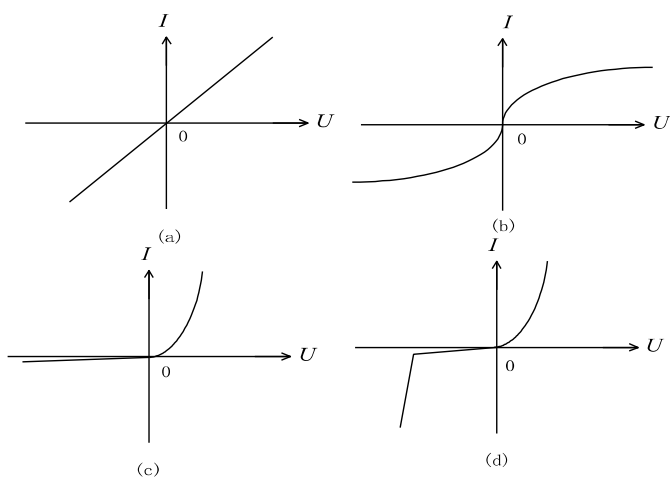
\includegraphics[width=13cm]{1.1.png} 
    \caption{各元件伏安特性曲线}
\end{figure}

\subsection{基尔霍夫定律的验证}

\section{实验设备}

\subsection{线性与非线性元件伏安特性的测绘}
\begin{enumerate}
    \item 直流电压、电流表
    \item 恒压源
    \item 电阻R=1000$\Omega$
    \item 半导体二极管1N-4007、稳压二极管\(2\text{CW}51\)(\(1\text{N}4728\))
    \end{enumerate}
\subsection{基尔霍夫定律的验证}

\section{实验内容及数据}
\begin{longtable}{cccc}
    %\centering
    \caption[Short Caption]{$支路电流数据$}
    \label{table:longtable_example} \\
    \hline
    支路电流(mA) & $I_{1}$     & $I_2$     & $I_3$     \\ \hline 
计算值      & 1.9256 & 5.988  & -7.913 \\ \hline
测量值      & 1.9554 & 6.005  & -7.930 \\ \hline
相对误差     & 1.55\% & 0.28\% & 0.21\% \\\hline
    \hline
\end{longtable}
\begin{longtable}{cccccccc}
    %\centering
    \caption[Short Caption]{$各元件电压数据$}
    \label{table:longtable_example} \\
    \hline
    各元件电压(V) & $U_{S_1}$    & $U_{S_2}$    & $U_{R_1}$    & $U_{R_2}$    & $U_{R_3}$    & $U_{R_4}$    & $U_{R_5}$    \\ \hline
    计算值      & 6     & 12     & 0.98   & 5.99  & -4.04   & 0.98   & 1.98  \\ \hline
    测量值      & 6.06  & 12.06  & 1.00   & 6.01  & -4.06   & 1.00   & 1.96  \\ \hline
    相对误差     & 1.00\% & 0.50\% & 1.83\% & 0.37\% & 0.60\% & 1.83\% & 0.81\% \\ \hline
    \hline
\end{longtable}
\end{document}